\documentclass[conference]{IEEEtran}
\IEEEoverridecommandlockouts
\usepackage{cite}
\usepackage{amsmath,amssymb,amsfonts}
\usepackage{algorithmic}
\usepackage{graphicx}
\usepackage{textcomp}
\usepackage{xcolor}
\usepackage{flushend}
\usepackage{array}
\usepackage{booktabs}
\usepackage{caption}
\usepackage{adjustbox}
\usepackage{tabularx}
\usepackage[section]{placeins}
\usepackage{balance}
\def\BibTeX{{\rm B\kern-.05em{\sc i\kern-.025em b}\kern-.08em
    T\kern-.1667em\lower.7ex\hbox{E}\kern-.125emX}}

\begin{document}

\title{Integrated Home Safety and Protection System\textbf{}}

\author{
\IEEEauthorblockN{\textit{Ha Thuc Quoc Hung, Pham Hoang Gia Huy, Nguyen Nhat Anh, Le Doan Gia Hung}}
\IEEEauthorblockA{\textit{FPT University, Ho Chi Minh Campus, Vietnam\\
Instructor: Duc Ngoc Minh Dang\\
\{htquochung.dev, giahuy250349, anhbin160304, lhung291005\}@gmail.com}}
}

\maketitle

\begin{abstract}
This paper presents a Smart IoT Home Security System developed on the ESP32 platform for real-time home monitoring, intrusion detection, gas leakage detection, and smart door control. The proposed system integrates an LDR sensor, MQ2 gas sensor, PIR motion sensor, and keypad as the primary input devices, while an LED indicator, buzzer, servo motor, and LED matrix are used as output modules. Sensor data are processed by the ESP32 through a continuous monitoring loop and event-driven decision logic. The system is connected to the Blynk IoT platform via WiFi to support remote monitoring, instant alert notification, and remote control functions. Experimental implementation indicates that the system can detect gas hazards, identify motion under low-light conditions, and manage password-based access control effectively. The developed prototype demonstrates a practical integration of embedded systems, multi-sensor fusion, and IoT communication for modern smart home security applications.
\end{abstract}

\begin{IEEEkeywords}
Smart home, ESP32, IoT, Blynk, gas detection, intrusion detection, home security
\end{IEEEkeywords}

\section{Introduction}
Smart home technology has become an important research direction because it enhances safety, convenience, and energy efficiency through interconnected sensing and control devices. Recent studies have shown that IoT-based home automation systems can support remote monitoring, intelligent decision-making, and distributed device management in residential environments \cite{malche2017internet,stojkoska2017review,gunawan2017prototype}. In particular, the integration of multiple sensors with cloud connectivity enables a home security platform to detect hazards more reliably and notify users in real time \cite{taiwo2021internet,al2020smart,iqbal2018interoperable}.

Motivated by these research trends, this project proposes a Smart IoT Home Security System using the ESP32 microcontroller as the central controller. The system combines gas detection, motion detection, ambient light sensing, and password-based door access in a unified architecture. Compared with a conventional single-function alarm system, the proposed solution applies multi-sensor fusion and context-aware logic, such as enabling intrusion detection primarily under dark conditions to reduce false alarms and improve practical usability \cite{gunawan2018performance,stojkoska2017review}.

The main objective of this work is to design and implement a compact embedded security system that supports both local control and Internet-based supervision. The system architecture, hardware connections, and logical workflow are presented through the block diagram, circuit diagram, pin connection tables, and programming flowchart in the following sections.

\section{Main Proposal}
The necessity of this topic arises from the increasing demand for low-cost, real-time, and remotely accessible home protection systems. Conventional household alarm systems often provide only local warnings, whereas modern IoT solutions can offer continuous supervision, mobile notifications, and flexible control \cite{taiwo2021internet,al2020smart}. Therefore, this project has both scientific significance in embedded IoT integration and practical significance in smart home deployment.

\subsection{System Model and Block Diagram}
The complete system is organized into four layers: input, processing, output, and IoT communication. In the input layer, the LDR detects ambient brightness, the MQ2 monitors smoke and gas concentration, the PIR detects human motion, and the keypad is used for password entry, reset, and password change operations. In the processing layer, the ESP32 collects sensor data, executes decision logic, maintains WiFi connectivity, and coordinates all actuators.

The output layer contains an LED, buzzer, servo motor, and LED matrix. The LED and buzzer indicate warning states, the servo motor acts as the smart door lock, and the LED matrix displays system messages. In the communication layer, the built-in WiFi module of the ESP32 exchanges data with the Blynk cloud server so that users can monitor sensor values and receive alerts through a mobile application.

\begin{figure}[!t]
\centering
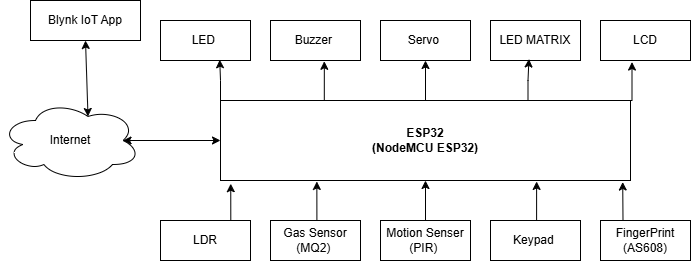
\includegraphics[width=\columnwidth,height=6.0cm,keepaspectratio]{BlockDiagram.png}
\caption{Block diagram of the Smart IoT Home Security System.}
\label{fig:block}
\end{figure}

\subsection{Components and Peripheral Devices}
The ESP32 is selected because it provides sufficient GPIO pins, built-in WiFi capability, low power consumption, and good compatibility with common embedded sensors. The LDR supports day and night context recognition. The MQ2 sensor is used because it can detect several combustible gases and smoke, making it suitable for household hazard monitoring. The PIR sensor provides reliable digital motion detection. The keypad offers a practical and low-cost local authentication interface. The servo motor performs door lock actuation after password verification. The LED, buzzer, and LED matrix provide immediate local feedback to the user.

Fig.~\ref{fig:devices} presents the hardware components used in the prototype based on the image files currently available in the project folder.

\begin{figure}[!t]
\centering
\setlength{\tabcolsep}{3pt}
\begin{tabular}{cc}
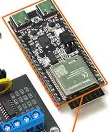
\includegraphics[width=0.46\columnwidth,height=2.6cm,keepaspectratio]{esp32.png} &
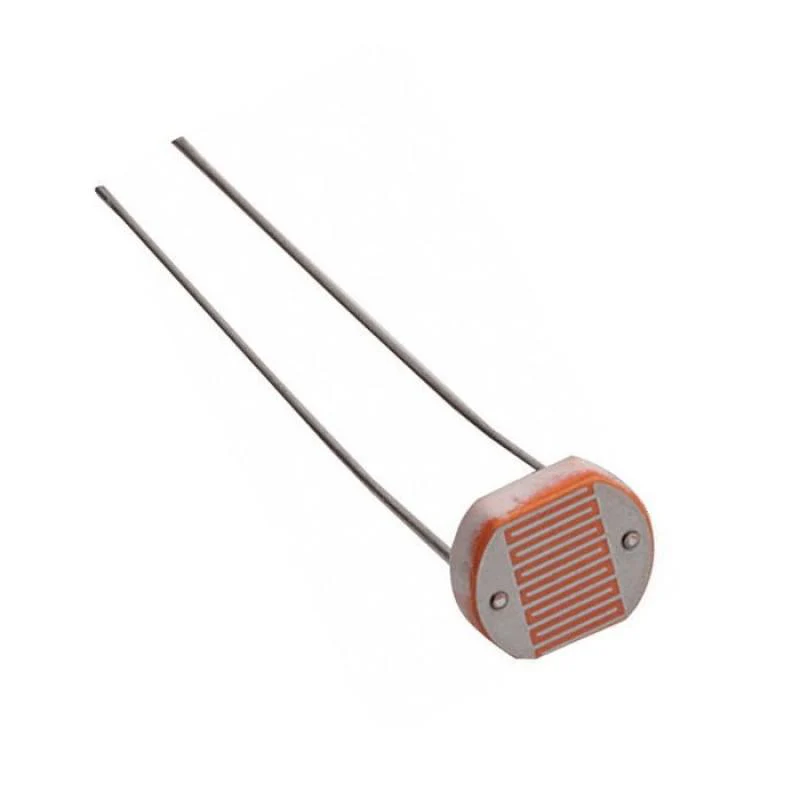
\includegraphics[width=0.46\columnwidth,height=2.6cm,keepaspectratio]{LDR.png} \\
ESP32 & LDR Sensor \\
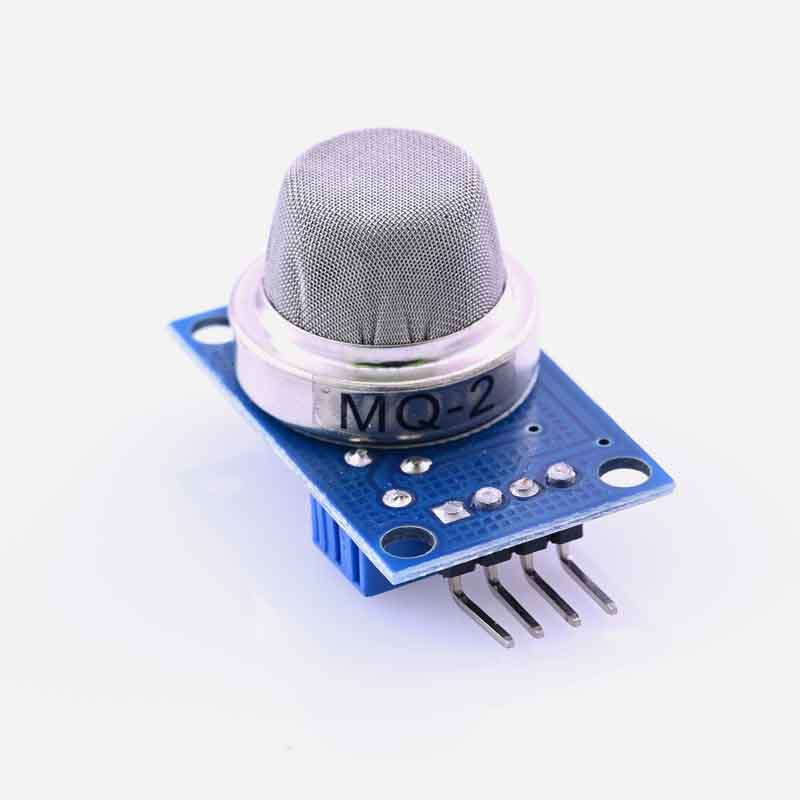
\includegraphics[width=0.46\columnwidth,height=2.6cm,keepaspectratio]{MQ2.jpg} &
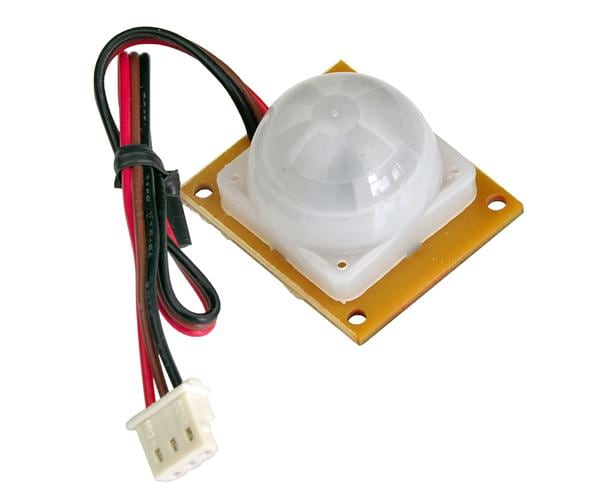
\includegraphics[width=0.46\columnwidth,height=2.6cm,keepaspectratio]{pir.png} \\
MQ2 Gas Sensor & PIR Motion Sensor \\
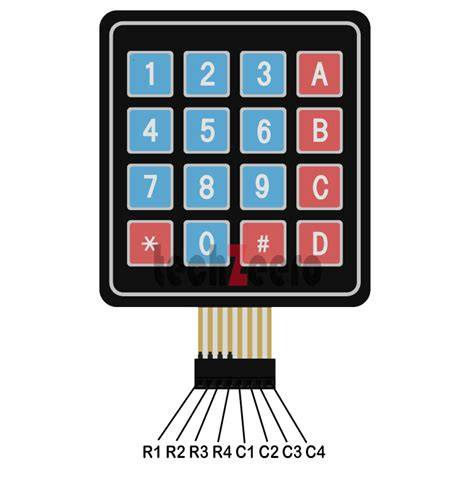
\includegraphics[width=0.46\columnwidth,height=2.6cm,keepaspectratio]{keypad.jpg} &
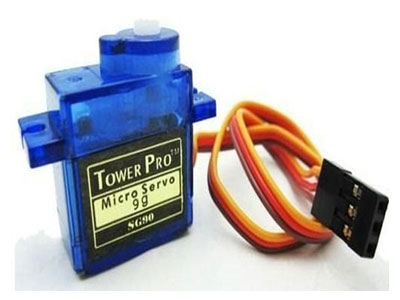
\includegraphics[width=0.46\columnwidth,height=2.6cm,keepaspectratio]{servo.jpg} \\
Keypad 4x4 & Servo Motor \\
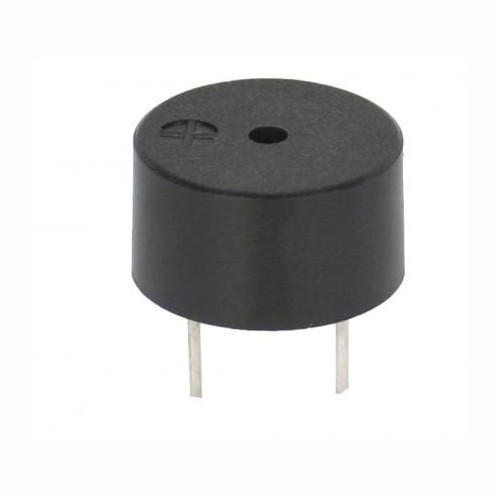
\includegraphics[width=0.46\columnwidth,height=2.6cm,keepaspectratio]{buzzer.png} &
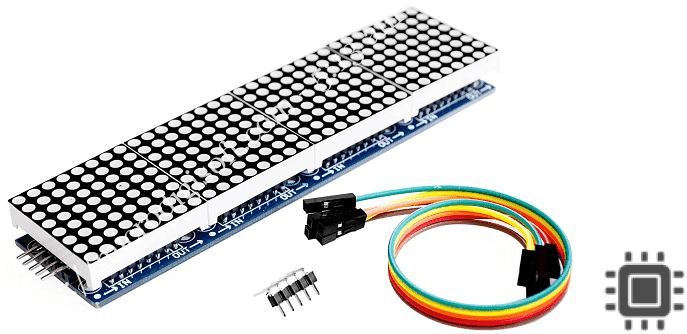
\includegraphics[width=0.46\columnwidth,height=2.6cm,keepaspectratio]{ledmatrix.png} \\
Buzzer & LED Matrix \\
\end{tabular}
\caption{Hardware devices used in the Smart IoT Home Security System.}
\label{fig:devices}
\end{figure}

\subsection{Circuit Diagram}
The circuit diagram illustrates the wiring relationship among the ESP32 controller, sensing modules, and output peripherals. Analog sensors such as the LDR and MQ2 are connected to the ADC-capable pins of the ESP32 for continuous monitoring. Digital modules including the PIR sensor, buzzer, servo motor, LED matrix, keypad, and optional fingerprint sensor are connected to dedicated GPIO pins according to their communication and control requirements. The complete circuit arrangement is shown in Fig.~\ref{fig:circuit}.

\begin{figure}[!t]
\centering
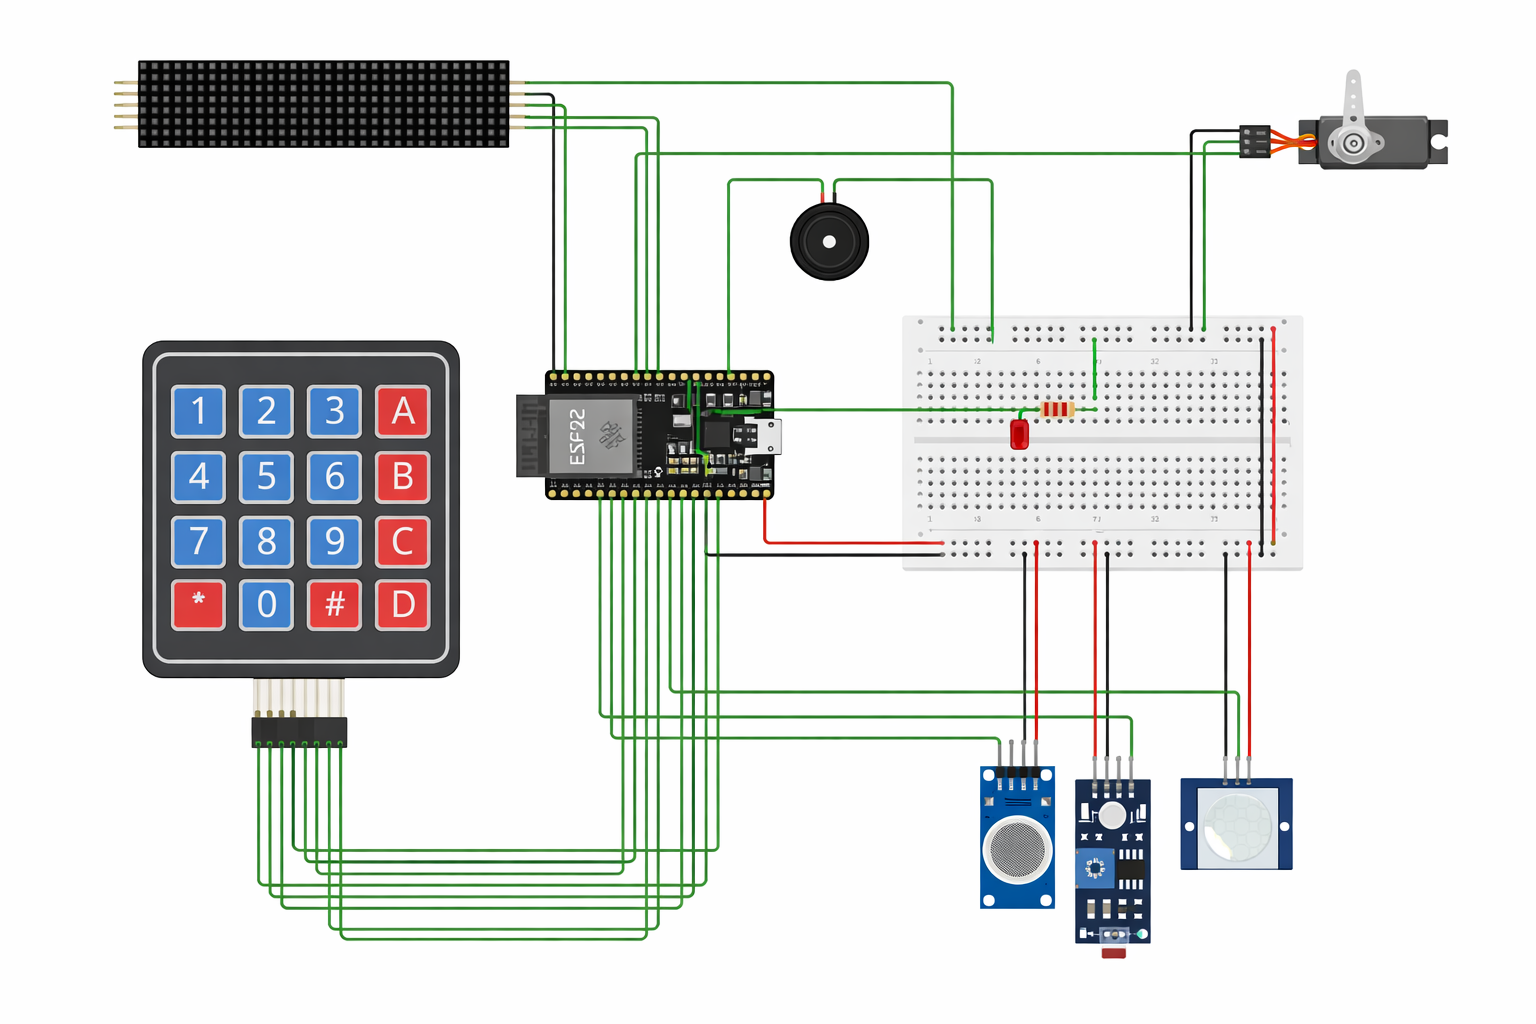
\includegraphics[width=\columnwidth,height=7.2cm,keepaspectratio]{circuitdiagram.png}
\caption{Circuit diagram of the Smart IoT Home Security System.}
\label{fig:circuit}
\end{figure}

\subsection{ESP32 Pin Connections with System Components}
Table~\ref{tab:pinmap} summarizes the proposed ESP32 pin assignments for the implemented prototype. Analog input pins are reserved for sensors that provide variable voltage levels, while digital output and communication pins are allocated to alarm modules, display modules, and authentication peripherals. In practical deployment, modules such as the MQ2 gas sensor, servo motor, and LED matrix should use an external 5~V supply with a common ground shared with the ESP32.

\begin{table}[!t]
\centering
\caption{ESP32 Pin Connections with System Components}
\label{tab:pinmap}
\scriptsize
\setlength{\tabcolsep}{3pt}
\renewcommand{\arraystretch}{1.15}
\begin{adjustbox}{max width=\columnwidth}
\begin{tabular}{|l|l|l|l|l|l|}
\hline
\textbf{ESP32 Pin} & \textbf{LDR} & \textbf{MQ2} & \textbf{PIR} & \textbf{Servo} & \textbf{Buzzer} \\
\hline
GND & GND & GND & GND & GND & GND \\
\hline
3V3 & VCC &  &  &  &  \\
\hline
5V/VIN &  & VCC & VCC & VCC & VCC (module) \\
\hline
GPIO34 & Analog output &  &  &  &  \\
\hline
GPIO35 &  & Analog output &  &  &  \\
\hline
GPIO27 &  &  & Digital output &  &  \\
\hline
GPIO19 &  &  &  & PWM signal &  \\
\hline
GPIO15 &  &  &  &  & Signal (+) \\
\hline
\end{tabular}
\end{adjustbox}
\end{table}

\begin{table}[!t]
\centering
\caption{Additional ESP32 Connections for Interface and Display Modules}
\label{tab:pinmap2}
\scriptsize
\setlength{\tabcolsep}{3pt}
\renewcommand{\arraystretch}{1.15}
\begin{adjustbox}{max width=\columnwidth}
\begin{tabular}{|l|l|l|l|l|l|}
\hline
\textbf{ESP32 Pin} & \textbf{LED Matrix} & \textbf{Fingerprint (AS608)} & \textbf{Keypad 4x4} & \textbf{LCD 16x2 (I2C)} & \textbf{RGB LED} \\
\hline
GND & GND & GND & -- & GND & Common anode (+) \\
\hline
5V/VIN & VCC & VCC & -- & VCC & -- \\
\hline
GPIO23 & DIN &  &  &  &  \\
\hline
GPIO18 & CLK &  &  &  &  \\
\hline
GPIO5 & CS &  &  &  &  \\
\hline
GPIO16 &  & RX of ESP32 from TX of sensor &  &  &  \\
\hline
GPIO17 &  & TX of ESP32 to RX of sensor &  &  &  \\
\hline
GPIO13, 12, 14, 4 &  &  & Row pins R1--R4 &  &  \\
\hline
GPIO26, 25, 33, 32 &  &  & Column pins C1--C4 &  &  \\
\hline
GPIO21 &  &  &  & SDA &  \\
\hline
GPIO22 &  &  &  & SCL &  \\
\hline
GPIO0 &  &  &  &  & RED (active LOW) \\
\hline
GPIO2 &  &  &  &  & GREEN (active LOW) \\
\hline
\end{tabular}
\end{adjustbox}
\end{table}

\subsection{Software Programming}
The software is implemented on the ESP32 using a continuous control loop. At system start-up, the controller initializes the sensors, output modules, WiFi connection, and Blynk communication channel. During runtime, the keypad input is read first for authentication and user management. If the entered password is correct, the servo unlocks the door for a predefined period and then automatically returns to the locked position.

After authentication handling, the system reads the MQ2 sensor value. If the gas level exceeds the safety threshold and the alert mechanism is enabled, the controller enters the gas alert state. In this state, the buzzer is activated, warning messages are shown on the LED matrix, and alert information is transmitted to the Blynk application. The controller also evaluates the PIR and LDR conditions together. When motion is detected in a dark environment, the system triggers an intrusion alarm by activating the LED and buzzer and sending a notification through the IoT platform. This decision logic demonstrates context-aware sensor fusion for more meaningful smart home behavior \cite{malche2017internet,iqbal2018interoperable}.

\subsection{Programming Flowchart}
The operational flowchart in Fig.~\ref{fig:flowchart} summarizes the system logic. The sequence begins with system initialization, WiFi connection, and Blynk cloud connection. The ESP32 then repeatedly performs four main tasks: reading keypad input, evaluating password conditions, reading gas concentration, and checking motion in dark conditions. If no abnormal event is detected, the controller remains in the normal monitoring state. Otherwise, it enters the corresponding alert state and activates the required outputs. This structure supports real-time response while keeping the overall program simple and reliable for embedded deployment.

\begin{figure}[!t]
\centering
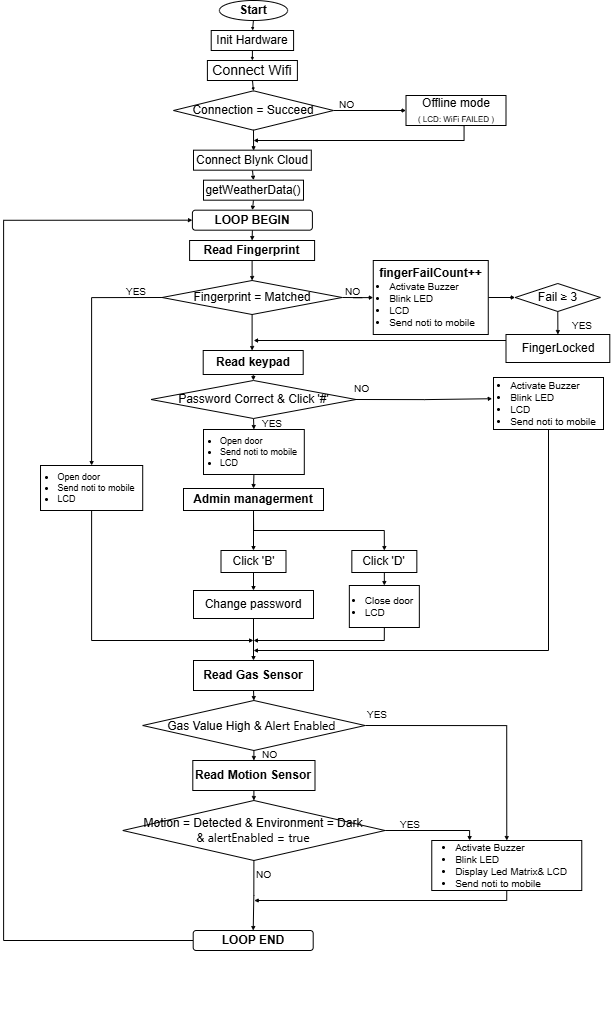
\includegraphics[width=\columnwidth,height=8.8cm,keepaspectratio]{Flowchart.png}
\caption{Programming flowchart of the developed system.}
\label{fig:flowchart}
\end{figure}

\section{Results and Discussion}
The prototype was implemented as an integrated embedded model using the ESP32, sensing modules, and local output devices. The design follows the practical direction of recent IoT smart home research, in which sensing, network communication, and remote supervision are combined into a compact and deployable solution \cite{gunawan2017prototype,taiwo2021internet}.

\subsection{Prototype Implementation}
The implemented system can monitor gas concentration, detect human motion, identify lighting conditions, and process user password input in real time. When the password is valid, the servo motor rotates to unlock the door. When gas concentration exceeds the threshold, the buzzer is activated and the warning state is transmitted to the mobile application. When motion is detected under dark conditions, the system interprets the event as a potential intrusion and triggers an alarm. The Blynk interface allows the user to observe sensor values, control selected functions, and receive notifications remotely.

\subsection{Blynk User Interface and Alert Notification}
The Blynk application serves as the main remote monitoring interface for the proposed system. Through the mobile dashboard, the user can observe real-time sensor values, check the operating status of the security system, and monitor alert conditions from a smartphone. In addition to dashboard visualization, the platform supports notification delivery when the gas sensor or motion sensor exceeds its trigger condition. Figures~\ref{fig:blynk-ui}--\ref{fig:mail-alert} present the reserved positions for the dashboard interface, in-app alert notification, and email notification generated by the system.

\begin{figure}[!t]
\centering
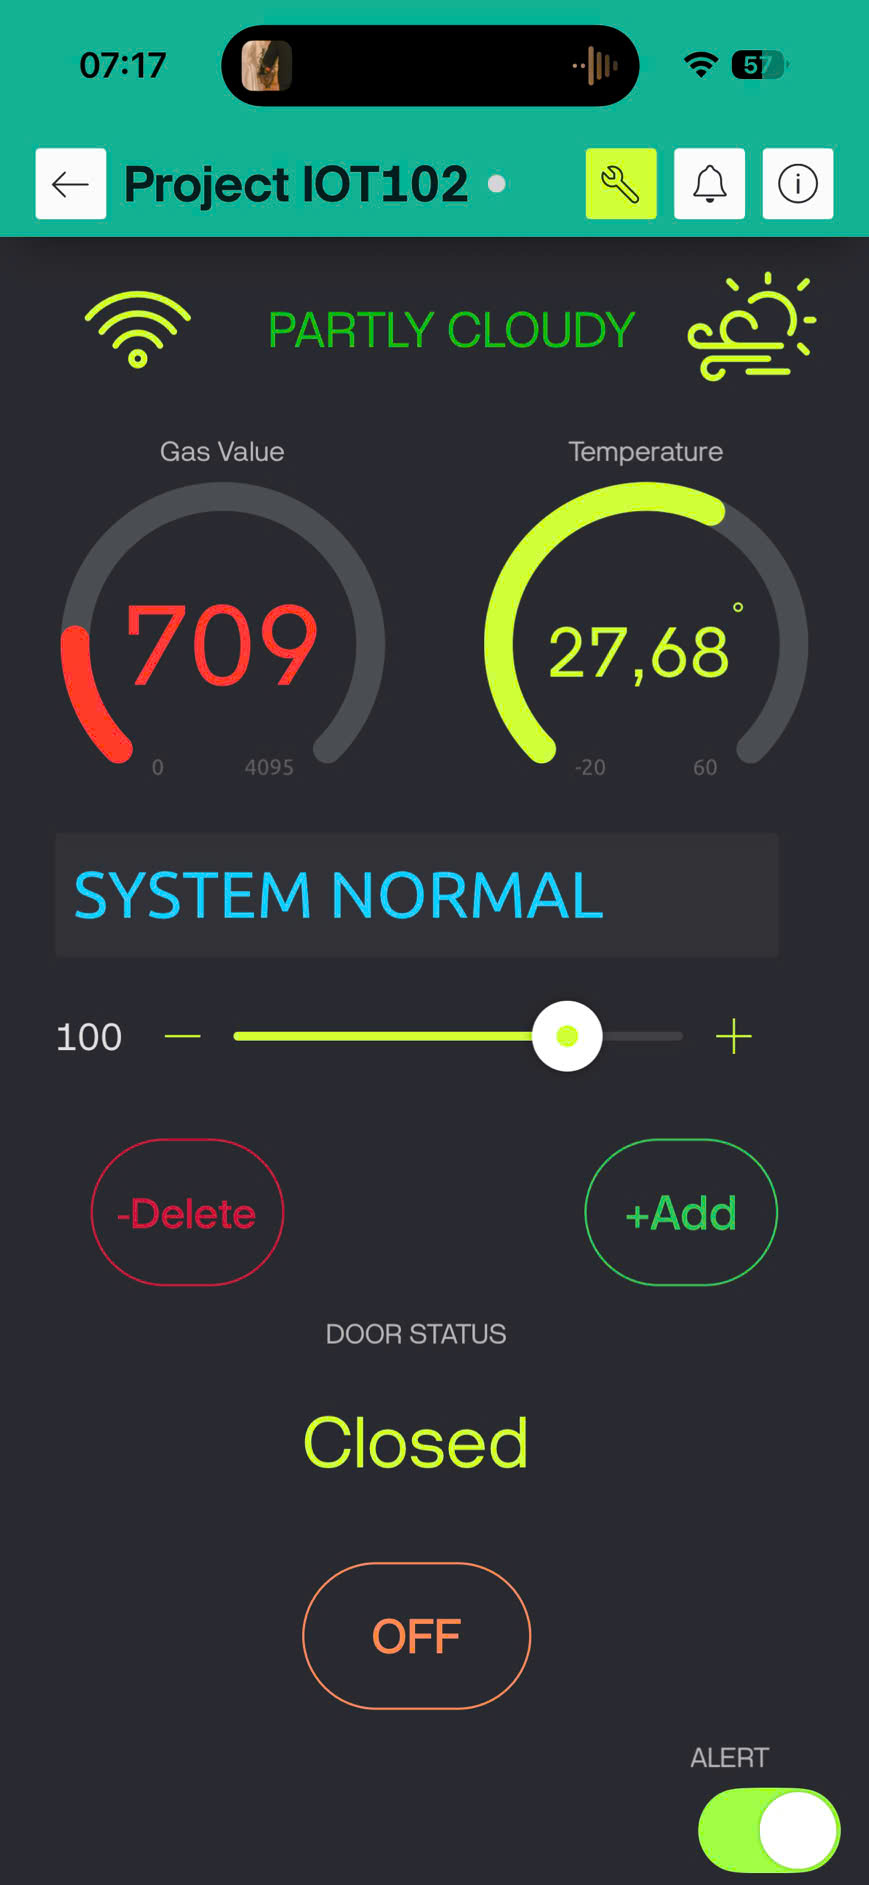
\includegraphics[width=0.78\columnwidth,height=5.8cm,keepaspectratio]{blynk_ui.jpg}
\caption{Blynk dashboard of the proposed system.}
\label{fig:blynk-ui}
\end{figure}

\begin{figure}[!t]
\centering
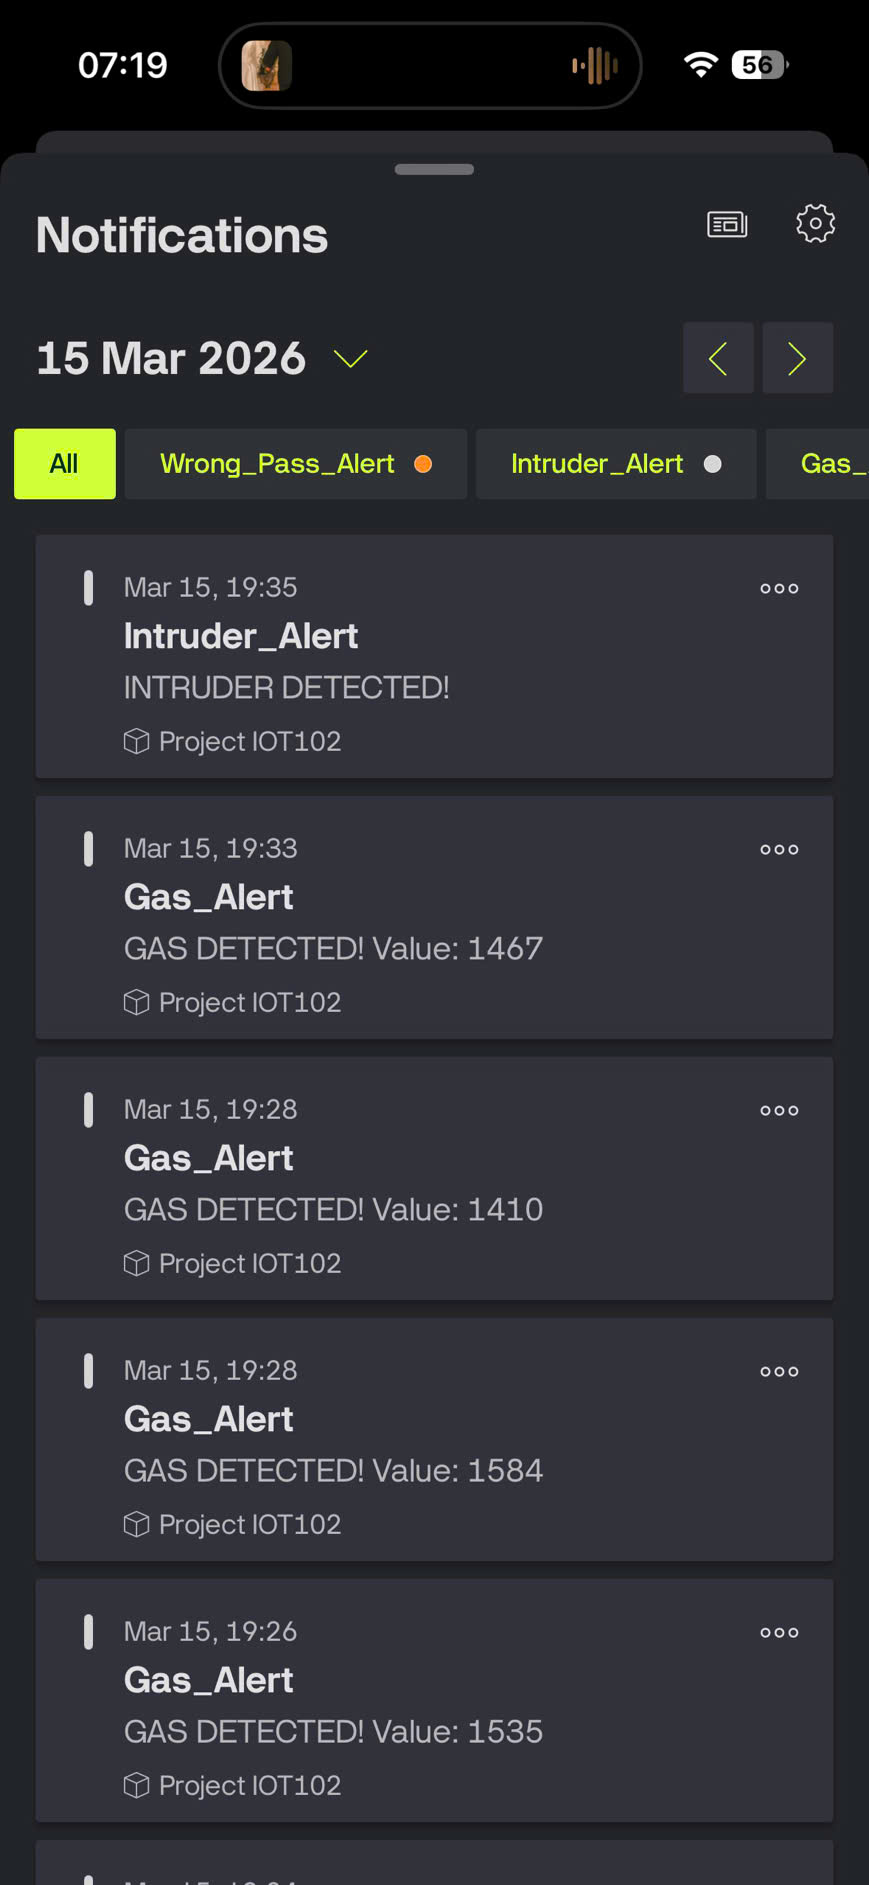
\includegraphics[width=0.78\columnwidth,height=5.8cm,keepaspectratio]{blynk_alert.png}
\caption{Alert notification displayed in the Blynk application.}
\label{fig:blynk-alert}
\end{figure}

\begin{figure}[!t]
\centering
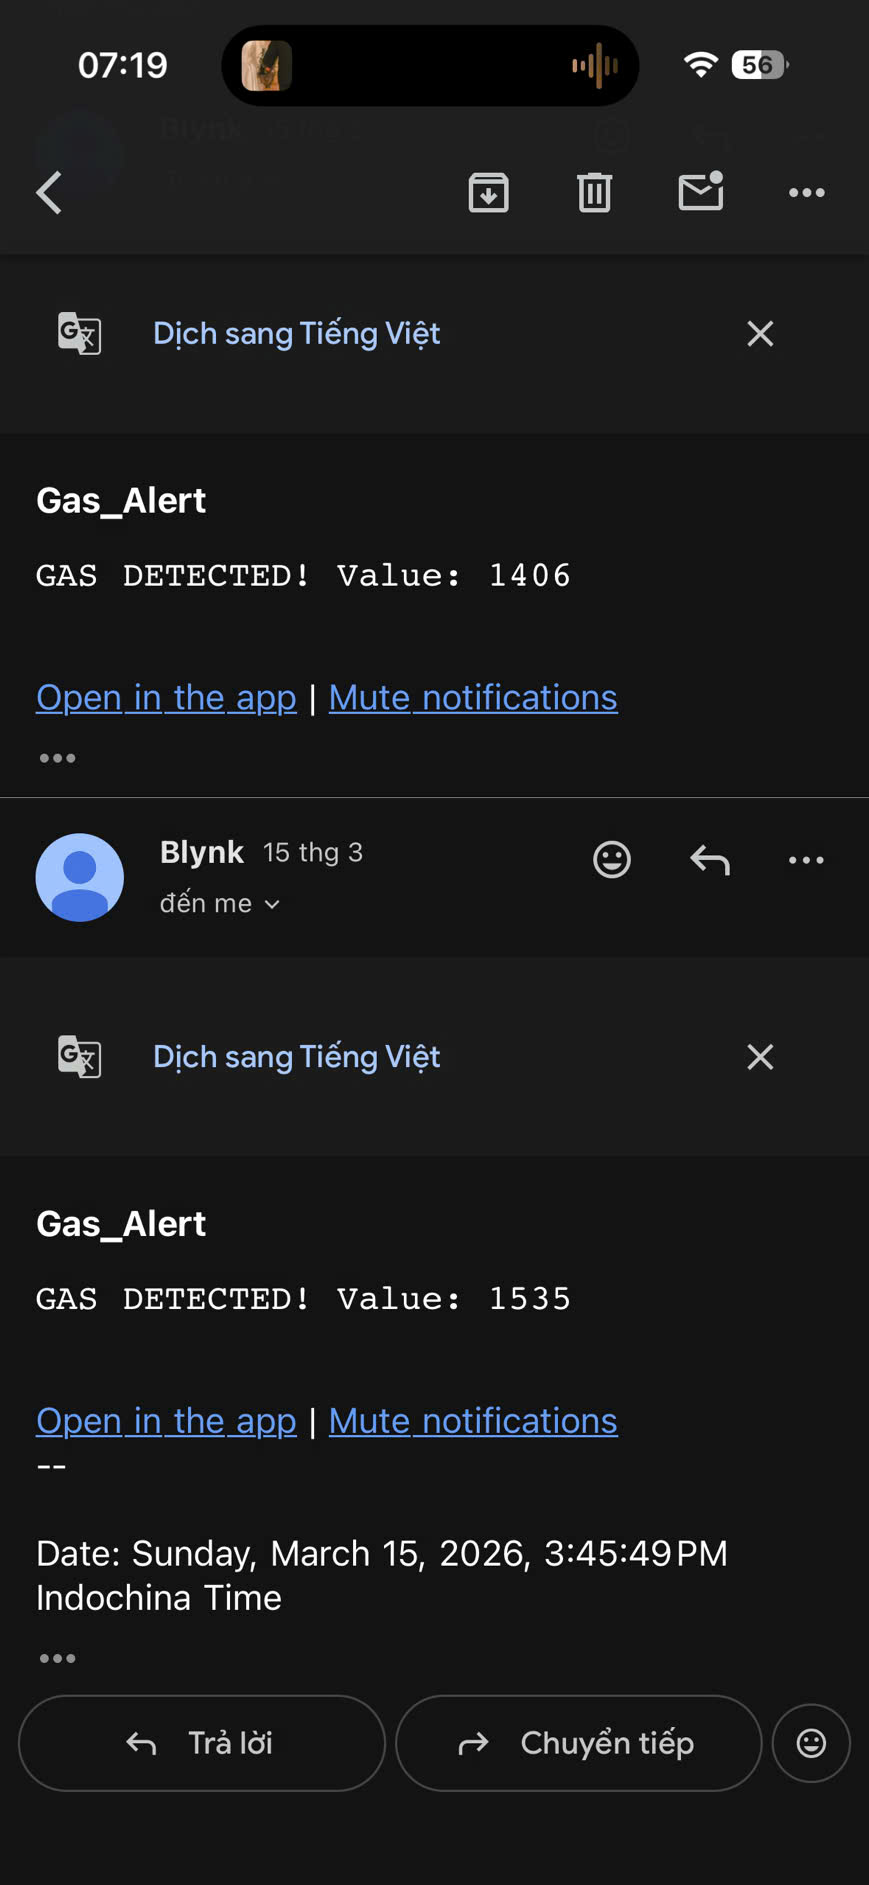
\includegraphics[width=0.78\columnwidth,height=5.8cm,keepaspectratio]{mail_alert.png}
\caption{Email notification generated when an alarm condition is detected.}
\label{fig:mail-alert}
\end{figure}

\subsection{Experimental Results}
The prototype achieved stable operation in repeated test scenarios. The MQ2 sensor successfully detected increased gas concentration and triggered the alert state. The PIR sensor responded effectively to movement, while the LDR helped reduce unnecessary alerts during bright conditions. Keypad-based authentication supported local access control and provided a simple method for changing or resetting the password. Remote synchronization through Blynk was maintained when WiFi was available, enabling mobile supervision of system status.

\subsection{Discussion}
The developed system provides several advantages. First, it combines multiple sensing functions in one platform, which improves flexibility compared with a standalone alarm device. Second, integration with Blynk increases convenience because the user can supervise the home from anywhere with Internet access. Third, context-aware logic helps reduce false positive motion alarms. However, some limitations remain. The system performance depends on WiFi availability, and low-cost sensors such as MQ2 and PIR may require careful threshold calibration in real environments. Future improvements may include biometric authentication, camera integration, data logging, and more advanced cloud analytics \cite{stojkoska2017review,gunawan2018performance}.

\section{Conclusion}
This paper presented a Smart IoT Home Security System based on the ESP32 platform for integrated home monitoring and protection. The system combines gas sensing, motion sensing, light sensing, password-based access control, and Internet-based notification in a unified embedded architecture. Experimental implementation confirmed that the prototype can operate as a practical smart security solution with real-time response, remote accessibility, and clear alert delivery through the Blynk platform. Overall, the project demonstrates the applicability of IoT technologies to safer and more intelligent residential environments \cite{al2020smart,taiwo2021internet,iqbal2018interoperable}.

\section{Author's Contribution}
\centering
\setlength{\belowcaptionskip}{2pt}
\captionof{table}{Author's contribution}
\label{tab:contribution}
\renewcommand{\arraystretch}{1.18}
\setlength{\tabcolsep}{2.2pt}
\scriptsize
\begin{adjustbox}{max width=\columnwidth}
\begin{tabular}{|>{\centering\arraybackslash}m{0.20cm}|>{\centering\arraybackslash\scriptsize}m{1.12cm}|>{\centering\arraybackslash}m{1.75cm}|>{\raggedright\arraybackslash}m{2.13cm}|>{\centering\arraybackslash}m{1.50cm}|}
 \hline
 \# & Student ID & Student Name & \centering Tasks & Contribution \tabularnewline
  \hline
 1 & SE191116 & Ha Thuc Quoc Hung & Study conception and program design; implement Arduino and ESP32 code; prepare presentation; draw block diagram and flowchart. & 30\% \\
  \hline
 2 & SE192041 & Pham Hoang Gia Huy & Study conception and system design; implement Arduino and ESP32 code. & 30\% \\
  \hline
 3 & SE192077 & Nguyen Nhat Anh & Draw flowchart and block diagram. & 10\% \\
  \hline
 4 & SE193449 & Le Doan Gia Hung & Write report; prepare presentation; draw block diagram and flowchart. & 30\% \\
  \hline
 \multicolumn{4}{|c|}{Total} & 100\% \\
 \hline
 \end{tabular}
\end{adjustbox}
\normalsize

\FloatBarrier
\bibliographystyle{IEEEtran}
\balance
\bibliography{Bib_references}

\end{document}
